% Chapter Template
%TODO section paragraphs
\chapter{Introduction}\label{introduction}
\section{Background on biological patterning}
\subsection{Morphogenesis in nature, examples and function}
%Periodic spatial structures in biology result from emergent phenomena where a tissue of cells gains heterogeneity and complexity in the spatial domain producing regular patterns.
%Spatial structures can be widely observed in nature both in \acrfull{2D} space such as the zebra's striped skin or in \acrfull{3D} in the labyrinthian brain cortex.

Periodic spatial structures in biology result when a tissue of cells gains heterogeneity and complexity in the spatial domain producing regular patterns.
Spatial structures can be widely observed in nature both in \acrfull{2D} space such as the zebra's striped skin or in \acrfull{3D} in the labyrinthian brain cortex.
Fig.~\ref{fig:pattern_examples} shows a wide variety of spatially periodic patterns encountered during my PhD thesis, which reflect how common these fascinating patterns are in different organisms and natural environments.
Although these patterns are extremely common, a mechanism to explain their robust assembly remains elusive to the scientific community.
Such interest stems both from a fundamental and an applied scientific point of view.
Understanding pattern formation in biology is key to getting a complete picture of how multicellular organisms grow from a single cell to a structure of organised cells with more complex functions.
In terms of applications, such understanding could enable tissue regeneration and engineering of tissues or organoids.

\begin{figure}[h!]
    \centering
    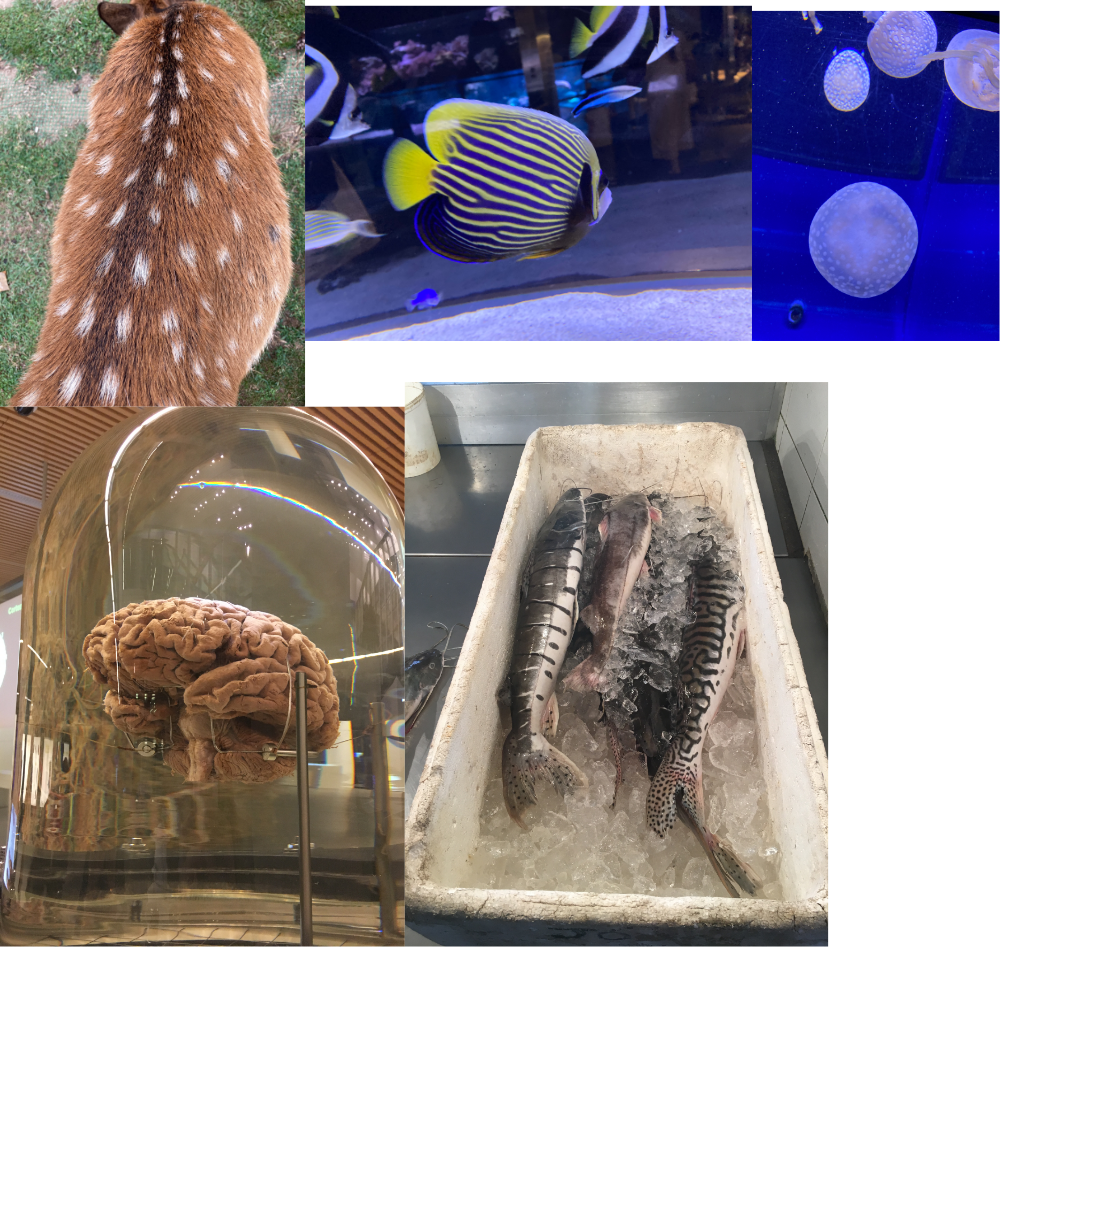
\includegraphics[width=1\textwidth]{chapters/Introduction/pattern_examples}
    \caption{\textbf{Examples of periodic patterns in biology.} Patterns observed during the course of this PhD study in molluscs, corals, mammals, plants, fungi, insects and fish. A wide variety of patterns including stripes, labyrinths and spots is displayed. Some organisms even display multiple patterns (e.g. pattern surrounding fish eye shows labyrinths, spots and stripes (F, top row, blue)}
    \label{fig:pattern_examples}
\end{figure}
This evolution from simplicity to complexity often plays a pivotal role in the functioning of multicellular beings.
More specifically, these patterns can have strategic advantages.
Fractal-shaped bacterial colonies, for instance, maximise nutrient absorption~\parencite{Matsushita1990}.
Furthermore, distinct colourations, such as the zebra's stripes or the mesmerising eye-spots on butterfly wings~\parencite{Blest}, serve to disorient predators; either by disrupting the prey's silhouette or suggesting the prey is part of a larger entity~\parencite{Stevens2006}.
The spirals observed in phyllotaxis offer plants a way to optimise sunlight capture, enhancing photosynthesis~\parencite{Strauss2020}.

The evolutionary advantage conveyed by this level of spatial organisation hints towards genetic networks being potentially responsible for such patterning mechanisms~\parencite{caro2005adaptive}.
A randomly found solution of evolution where a pattern occurs could lead to the genetic networks driving these spatial arrangements to be evolutionary beneficial and therefore selected. %TODO What is a randomly found solution of evolution?
Comprehending these networks and the dynamics that lead to these spatial designs is essential.
This area of research not only tries to understand which genetic networks and mechanisms are behind patterning.
It also seeks to uncover how on a molecular scale these mechanisms are reliable, accurate and robust to the noisy and exposed biological environment.

Additionally, the study of pattern formation extends well beyond the realms of developmental biology and morphogenesis.
It lays the groundwork for innovative advancements in biotechnological sectors.
This includes enabling the creation of intricately patterned tissues, efficient biofilms, and potentially even organoids with significant implications in groundbreaking applications like tissue regeneration and organ implants~\parencite{Scholes2017}.
The field's promise is further evidenced by existing applications, such as polyamide membranes featuring periodic Turing structures for water purification~\parencite{Tan2018}, showcasing the practical potential of these developments.

\subsection{Patterning theories}
Numerous mechanisms have been proposed in the literature to explain pattern formation in biological systems.
Some of the most relevant ones can be categorized into physical and diffusion-based mechanisms~\parencite{hiscock2015mathematically, Scholes2017}, as seen in Fig.~\ref{fig:physical_based_mechanisms} and Fig.~\ref{fig:diffusion_based_mechanisms} .
Physical-based methods involve models where physical forces play an important role.
Some mechanisms in this category include phase separation, which can occur through differential cell adhesion , wrinkling, which can occur through mechanical instabilities, or branching (Fig.~\ref{fig:physical_based_mechanisms}).
For example, forces and tissue mechanics are important for patterning villi in the gut, as seen in Fig.~\ref{fig:physical_based_mechanisms}A (left)~\parencite{shyer2013villification}, while differential cell adhesion is key for the self-assembly of pancreatic islets~\parencite{jia2007tissue}.
On the other hand, diffusion-based mechanisms rely on cells in the tissue responding to a molecule that is spatially heterogeneous and therefore exhibits different phenotypes in different regions of the tissue.
Among these gradient-based mechanisms, notable examples include the positional information model and the Turing model~\parencite{Wolpert1969, Turing1952}, as seen in Fig.~\ref{fig:diffusion_based_mechanisms}.
The focus of this thesis is on diffusion-based mechanisms, and we will therefore explore these more in detail.

\begin{figure}[H]
    \centering
    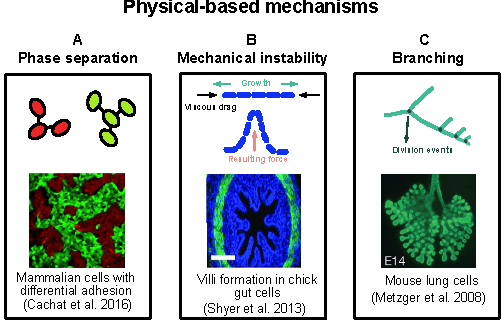
\includegraphics[width=1\textwidth]{chapters/Introduction/physical_based_mechanisms}
    \caption{\textbf{Patterning mechanisms in biology.} \textbf{(A)}
    Phase separation can occur through different mechanisms including differential cell adhesion where different cell types bind to themselves. An example is the syntheticly engineered patterns with differential cell adhesion. Image from~\cite{cachat20162}.  \textbf{(B)} Mechanical instability can occur through combined forces, as in the wrinkling of villi in the gut, where growth can generate perpendicular forces that deform the tissue. Image from~\cite{shyer2013villification}.
    \textbf{(C)} Branching can occur through local cell division events which lead to tree-like structures in the lung. Image from~\cite{metzger2008branching}.}
    \label{fig:physical_based_mechanisms}
\end{figure}
%TODO add externally controlled below PI and self-organised below Turing

\begin{figure}[h]
    \centering
    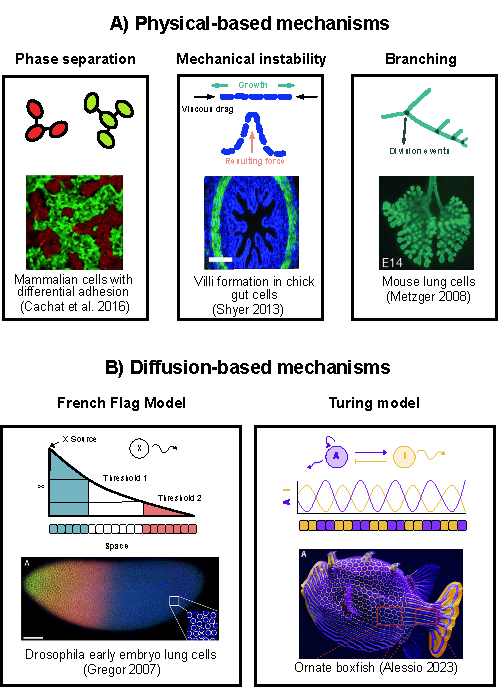
\includegraphics[width=1\textwidth]{chapters/Introduction/diffusion_based_mechanisms}
    \caption{\textbf{Patterning mechanisms in biology.} \textbf{(A)} Positional information occurs with a gradient of morphogen X, steaming from a source. This gradient is then interpreted by cells forming three different gene expression regimes and phenotypes (green, pink, blue).
    The example shows an early drosophila embryo stained for DNA (blue), Hunchback protein (red), and Bicoid protein (green) with three partitioned regions. Image from~\cite{gregor2007probing}. \textbf{(B)} The Turing mechanism involves a network with a slow diffusing activator (purple) and a fast diffusing inhibitor (yellow). When they interact, they form a periodic stationary pattern which can lead to spatial spots, stripes or labyrinths in biology as seen in the Ornate boxfish. Photo courtesy of the Birch Aquarium at the Scripps Institution of Oceanography.}
    \label{fig:diffusion_based_mechanisms}
\end{figure}



\subsection{Wolpert's Positional information versus Turing's Reaction-Diffusion}
The positional information, also called the French-Flag model, is underpinned by an initial gradient of morphogens, interpreted by a genetic network to induce tissue patterning ~\parencite{Wolpert1969}.
Morphogens are signalling molecules which can act over long distances, classically by diffusion, and induce responses in the cells such as activation of gene expression~\parencite{rogers2011morphogen}.
Sometimes, the origins of this morphogen gradient can be attributed to external factors such as ambient temperature, maternal impacts, or light exposure~\parencite{Schier2009}.
A simple genetic network interpreting this gradient can partition the tissue into three regions where the first region (green) appears for concentrations of morphogen above Threshold 1, and the third region (blue) results for concentrations below Threshold 2 (Fig.~\ref{fig:diffusion_based_mechanisms}A (top)).
An example of positional information occurs in the drosophila embryo, where different gene expression domains are generated by the bicoid gradient (Fig.~\ref{fig:diffusion_based_mechanisms}A (bottom)).
In this case, the mother acts as a source by providing bicoid mRNAs in the anterior of the fly, which diffuse towards the posterior, generating different gene expression profiles ~\parencite{grimm2010modelling}.

Positional information has several caveats.
The number of repeats does not scale up with tissue size, meaning bigger tissues have the same number of peaks with a larger wavelength.
Therefore the periodicity observed in some biological systems cannot be replicated.
Additionally, in specific instances, the presence of an initial pre-pattern might be implausible, raising questions about how patterns spontaneously emerge from a prior uniform tissue.
Addressing these conundrums, the Turing's model offers an alternative which provides scaling of repeats where the wavelength remains constant for larger tissues as more peaks arise.
Additionally, it does not need a pre-existing gradient and is self-organising~\parencite{Turing1952, Kondo2010a}.

This mechanism is based on a simple network with a slow-diffusing activator and a fast-diffusing inhibitor which interact together to generate an emergent periodic pattern.
An example of this is shown in Fig.~\ref{fig:diffusion_based_mechanisms}B (top) where the concentrations of the two molecules, A and I, form an out-of phase spatial wave.
In two dimensions, the Turing model results into complex patterns such as labyrinths, spots and stripes observed in many organisms including the Ornate Boxfish ~\parencite{Alessio2023} (See Fig.~\ref{fig:diffusion_based_mechanisms}B (bottom)).

Over the past 70 years, the acceptance of Turing's \acrfull{RD} model and Wolpert's positional information theory in developmental biology has evolved significantly~\parencite{green2015positional}.
When Turing's reaction-diffusion model was introduced in 1952, it did not gain traction within the biological community due to various reasons.
Originally, it was a theoretical concept with limited empirical evidence as the field of molecular and developmental biology was still not very advanced.
Additionally, the theory was presented on a complex mathematical framework which was hard to understand and which described an overly simplistic and rigid network that did not reflect biological complexity.
When Wolpert's positional information was introduced in the 70's, it immediately became popular and was established as the dominant paradigm in the field of developmental biology.
It provided a conceptual framework which was easier to grasp and which could be directly applied to the observations and experiments in developmental biology such as the growth of limb buds in the chick embryo~\parencite{saunders1968ectodermal}.
The concept of reaction-diffusion, previously introduced by Turing, was revived in 1972 by Gierer and Meinhardt, who proposed a refined version of Turing's model, addressing some of its limitations and making it more biologically plausible.
Additionally, they introduced the general principle of "short range activation, long range inhibition", which made Turing's RD model more intuitive.
It is important to mention that while Turing's results were calculated by hand, Gierer and Meinhardt's calculations were done using computers.
These advances in computer technology along with progress in molecular biology also allowed a better understanding of reaction-diffusion models which began to attract attention.

Given its attributes, the reaction-diffusion model might provide a more complete answer to the question of patterning in biology and more holistic perspective on the intricacies of morphogenesis.
For this reason, Turing mechanism for pattern formation will be the main focus of this work.
Nevertheless, it is pivotal to recognize that these mechanisms are not strictly independent of each other (e.g. digit formation has morphogen gradients, while it is likely a Turing mechanism~\parencite{Raspopovic1}).
The intricate nature of biological patterning might be best elucidated by an amalgamation of these theories, suggesting a blended framework may hold the answers~\parencite{Green2015}.
%TODO if time, comment on clock and wavefront model Baker2006
%%%%%%%%%% corrected up to here

%todo discuss Turings comment Turing himself recognized the biological unreality of this in stating that 'most of an organism, most of the time is developing from one pattern to another, rather than from homogeneity into a pattern' 1-34]


\section{Reaction-diffusion systems}
\subsection{Turing patterns}
Reaction-diffusion systems were originally introduced in 1952 by Alan M. Turing in his paper “The chemical basis of morphogenesis”~\parencite{Turing1952}.
In this article, he argues that pattern formation can be obtained when two morphogens interact with each other and diffuse at different
velocities across a tissue.
If these morphogens can activate the production of growth hormones or skin pigments, biological patterns leading to a phenotype can arise.
The resulting patterns, called Turing patterns (TPs), can have different shapes such as stripes, labyrinths, spots; which can be widely observed in natural systems.
The concept of Turing patterns was first introduced from a mathematical perspective and was modelled using space and time dependent partial differential equations (PDE). In the case of Turing’s seminal paper, the set of PDEs describes a two node network (Fig.~\ref{fig:intro_to_Turing_patterns}A) which has activation and inhibition terms, degradation terms and diffusion terms (Fig.~\ref{fig:intro_to_Turing_patterns}B).
The key feature of this system is that it can exhibit diffusion driven instabilities: Initially, the tissue has a homogeneous concentration of morphogen under which no diffusion occurs, and under these circumstances the system is stable and converges into an equilibrium state.
When biological noise is introduced, the heterogeneity of the system leads to morphogen diffusion.
Consequently, the diffusion leads to changes in the reaction rates and the system is pushed out of steady state leading to an unstable system.
This unstable system converges into a stable stationary periodic pattern which is a Turing pattern (Fig.~\ref{fig:intro_to_Turing_patterns}C).
This whole phenomenon, called the diffusion-driven instability, is the essence of Alan Turing’s paper and one of the most used mechanisms to explain morphogenesis.

\begin{figure}[h!]
    \centering
    \includegraphics[width=1\textwidth]{chapters/Introduction/intro_to_Turing_patterns}
    \caption{\textbf{Introduction to Turing mechanism of pattern formation}. \textbf{(A)} two node network based on Turing's original paper. Slow diffusing activator in green and fast diffusor inhibitor in pink. \textbf{(B)} Linear PDE equations for a two-node Turing system. \textbf{(C)} 2D simulation of equations in (B). \textbf{(D)} Here we display the mechanism of pattern formation with an activator-inhibitor system for an in-phase pattern. The system starts with a homogeneous distribution of activator an inhibitor (Time 1). However, this apparent homogeneous distribution, exhibits molecular fluctuations where the activator prevails over the inhibitor (Time 2). In this point in space, activator (green) is auto-enhanced, amplyfing such perturbations. Since the activator also enhances the inhibitor (pink), its levels will also rise in this region (Time 3). Finally, the inhibitor diffuses further away than the activator leading to two outcomes. Neighbouring regions to the peak go through repression and therefore concentrations of both molecules drop. Additionally, due to its fast diffusion, levels of inhibitor in the peak are not high enough to repress the activator  (Time 4). This leads to an organised system of peaks and troughs of molecule concentration which dynamically settles into a stationary pattern.}
    \label{fig:intro_to_Turing_patterns}
\end{figure}
%\frac{\partial A}{\partial t} = 5A - 6I + 1 - D_{A}\nabla^2 A
%\frac{\partial I}{\partial t} = 6A - 7I + 1 - D_{A}\nabla^2 A
%TODO rerun simulations  1D snapshots and video


%TODO change diagram to add  https://journals.biologists.com/dev/article/142/7/1203/47299/Positional-information-and-reaction-diffusion-two Fig1
\subsection{Gierer-Meinhardt model}
Although Turing’s work was of key importance in the field of developmental biology, it was not well accepted by biologists due to various reasons.
Firstly, the mathematical complexity behind it made it non-intuitive for many scientists in the field and hard to explore due to the lack of computers.
Furthermore, the network proposed, although it can generate patterns, is too simple to describe the complexity in biological systems and produces some unrealistic results such as the presence of negative concentrations due to the lack of non-linearities~\parencite{Kondo2010a}.
To solve these two issues, Gierer and Meinhardt proposed a generalised version of Turing’s diffusion-driven-instabilities~\parencite{Gierer1972}.
This alternative theory proposes that patterns can be obtained as long as short-range activation and long-range inhibition (SALI) are present.
This implies that we can go away from Turing’s equations and extend the theory to networks with different number of nodes, different network interactions and even different signal transduction mechanisms~\parencite{Murray1983, Rauch2004, Swindale1980}.
This step was necessary to be able to attribute patterning phenomena to more complex cellular and molecular interactions described by non-linear terms and larger networks with more nodes involved.
Examples of the first systems developed with non-linear terms are the typical Gierer-Meinhardt model~\parencite{Gierer1972}, Schnakenberg model~\parencite{Schnakenberg1979}, as well as the Thomas model~\parencite{thomas1976analysis}.
This generalisation work sheds some light into the logic behind patterning and allows to understand it intuitively: as an initially homogeneous system is perturbed by biological noise, local peaks of a morphogen concentration form.
These transient peaks lead to a local activation effect where the concentration of all reactants increases.
Due to the difference in diffusivity, the inhibitor reaches further away and long range inhibition is achieved.
Ultimately, this system settles into a stationary pattern with activation peaks and inhibition troughs~\parencite{Gierer1972}.
This SALI mechanism proposed in this paper is shown in Fig.~\ref{fig:intro_to_Turing_patterns}D.
%todo maybe add more detail from detailed explanation: Imagine a system with two chemicals: an activator and an inhibitor. The activator stimulates its own production, that of the inhibitor, and the production of black pigment. The inhibitor, however, reduces the production of both activator and black pigment.This simple network leads to regular patterns when diffusion is introduced: these chemicals can spread, but they do not travel at the same speed. The activator moves slowly, affecting only nearby areas, while the inhibitor travels faster, reaching farther areas. As the activator starts working, a local region of black is produced. Some inhibitor is also produced, which travels faster than the activator, reaching further away and leading to inhibition and white in the areas surrounding the black. Once the inhibitor's effect diminishes in a distant region, the activator becomes dominant again, leading to another spot of pigment production. The repetition of this event across the tissue results in regular spots or stripes of pigment. These are the principles underpinning Alan Turing’s theory of pattern formation known as “Turing patterns”, which explain regular pattern formation in biology.

\subsection{Turing patterns in nature}\label{Turing patterns in nature}
Various links have been made between biological patterns found in nature and Turing patterning networks.
As a basic example, seashell pigmentation and various types of fish skin have been replicated using simulations of Turing pattern systems.
Additionally, perturbation experiments in zebrafish’s skin are consistent with simulations of RD equations where the pattern regenerates in the exact same way after being physically disrupted both \textit{in-vivo} and \textit{in-silico}~\parencite{Kondo2010a}.
Perturbation experiments are also carried out in the mammalian palate, providing evidence of a Turing-type reaction-diffusion mechanism~\parencite{Economou2012}.

From a molecular biology point of view, molecules involved in patterning and morphogenesis have been shown to be part of networks with SALI characteristics.
For example, hair follicle development and fingerprint formation have been shown to rely on the same Turing reaction-diffusion network, based on signaling between WNT and BMP~\parencite{Glover2023}.
In this case, WNT is the activator while BMP is the inhibitor.
WNT directly promotes cell proliferation and indirectly hair follicle generation through synergy with the EDAR pathway.
Therefore, in the presence of WNT, there will be growth and hair follicle formation.
WNT distribution in space is periodic, likely due to a Turing mechanism, and therefore forms periodic hair follicle formation and ridges in the fingerprints.
Other examples of Turing SALI networks are Nodal \& Lefty in right left asymmetry~\parencite{Nakamura2006} and finally Wnt \& Dkk involved in lung branching~\parencite{langhe2005_lung}.
All these examples of the relationship between biological patterns and RD systems, SALI networks and diffusion-driven instabilities strongly suggest that the Turing mechanism is linked to the self-assembling and self-regenerative patterns observed in nature.

However, the arguments mentioned above make Turing’s mechanism purely a strong hypothesis of patterning and do not prove causation.
This is because obtaining a 2D solution that matches the experiments does not necessarily mean the model used is the correct one.
Furthermore, the involvement of a Turing-type network in patterning does not discard the possibility of an interplay of multiple mechanisms contributing to this organization.
For instance, Bmp, Sox9, and Wnt constitute a Turing network involved in the development of limb digits, as proven by ~\cite{Raspopovic1}.
However, the presence of an Shh gradient in the limb bud suggests this developmental programme could arise from a combination of Turing's reaction-diffusion and Wolpert's positional information.
%TODO comment on the only way of proving this mechanism is responsible is synbio

%todo Feather patterning appears to similarly combine these mechanisms - reaction diffusino with cell movement (Ho et al.,2019).

\section{Mathematical analysis of Turing patterns}

\subsection{Mathematical methods to study Turing patterns}
Turing patterns are commonly studied using mathematical tools to understand their features and behaviours.
The equations describing these reaction-diffusion systems are usually too complex to solve analytically as they contain non-linearities and partial differential terms.
For this reason, different methods must be used such as \acrfull{LSA} or numerical methods.

LSA provides information on how the stability of the system evolves as we go from a system without diffusion to a system with diffusion~\parencite{Glendinning1994}.
For RD systems to produce Turing patterns, they must be stable without diffusion and become unstable as diffusion is turned on~\parencite{J.DMurray2002}.
This stability profile gives rise to the name \acrfull{DDI} which is an alternative name for Turing patterns.
In principle, this method can tell us whether a system is a pattern generator but does not provide a solution of the pattern in space and time. Additionally, because the system is linearised around the steady state, non-linear terms or multistability might alter the final outcome.
More information on how LSA is used to understand patterning and DDI's is found on Section~\ref{lsa} in the following chapter.

Alternatively, numerical methods are used to calculate the concentration of species in the RD system at every time and space point~\parencite{Ramos1983}.
A visual solution is obtained which provides information on the shape, wavelength, evolution and amplitude of the pattern.
While numerical methods provide more information than LSA, they are more computationally expensive and can lead to numerical errors~\parencite{J.DMurray2002}.
Various numerical solvers exist for this purpose, but after much research,~\acrfull{CN} for~\acrshort{1D} space and~\acrfull{ADI} for~\acrshort{2D} space were considered the most adequate in terms of speed and accuracy for this project (See Section~\ref{numerical_methods}).
To explore and get intuition on the numerical solutions of a system, recently developed online tools such as VisualPDE can be used before studying the problem in detail with other solvers~\parencite{Walker2023}.
Both numerical and analytical tools have their advantages or disadvantages and must be used in combination for an optimal study of RD systems and patterning.

\subsection{The robustness problem}

Using both linear stability analysis and numerical methods, Turing patterns were widely studied to understand whether they were a plausible explanation for pattern formation in biology.
Although patterns were obtained analytically and numerically using models of the SALI networks mentioned above, the robustness problem makes this mechanism questionable.
The robustness problem or the fine-tuning problem refers to the small fraction of the parameter space leading to Turing patterns and high sensitivity to parameter changes.
For example, original 2-node reaction-diffusion systems require large differential diffusion rates between the two morphogens as explained previously for SALI mechanism to occur.
If this constraint in parameters is not met, the robustness for pattern formation is highly reduced.
Achieving this differential diffusivity experimentally is sometimes biologically unlikely, as many of the morphogens have similar diffusion rates due to their similarities in molecular size~\parencite{huidobro}.

The robustness issue was explored in detail in~\cite{Scholes2019} using an atlas approach, where the parameter space of all 2-node and 3-node networks were studied using LSA to check for Turing patterning.
The atlas study involves constructing all possible networks using adjacency matrices, where a -1 represents an inhibition edge from one node to another, 0 represents no interaction and +1 represents an activation.
All 2x2 and 3x3 adjacency matrices are created and network symmetries are checked to remove homologous networks.
By carrying out LSA on the resulting networks, it was found that although 61\% of the networks can produce Turing patterns, only 0.1\% of the parameter space is within Turing space.
Similar results were obtained in~\cite{Zheng2016} and~\cite{Marcon}.


Another issue with Turing patterns is the sensitivity to the initial conditions.
Although the shape of the pattern is not strictly determined by the initial conditions, finer details like locations of spots and stripes can be influenced.
Additionally, although the final pattern is the same, the transient dynamics might differ between different initial conditions (e.g. different transient pattern or convergence time before settling into the final pattern).
This can be an issue as in developmental biology, is a tightly controlled process where cells must receive the exact same signals in the same location and time to robustly reproduce the pattern. %todo find ref for this.





\subsection{Robustness of Turing patterns in realistic systems: larger networks, growth, boundaries, noise, agar thickness}
On one hand, Turing's mechanism seems to explain many different patterns in biology as well as their perturbation experiments.
On the other hand, it does not seem like a very robust mechanism.
How do these two contradicting ideas come together?
How can we make patterns more robust?
Typically, Turing patterns are often studied in non-realistic systems.
A new direction in the field aims to study Turing patterns in more realistic systems and see how these effects affect robustness.

%large networks, systems with cooperativity, tissue discreteness at the cell level, growth, different boundary conditions, noise, delays, agar thickness.
%Surprisingly, some of these realistic biological conditions increase robustness for Turing pattern formation. %Studying Turing patterns with a more biological point of view can potentially help solve the robustness issue.

\subsubsection{Large networks}
Biological networks are usually far from the idealised 2-node Turing networks. %todo quote average network size
Recent studies~\parencite{Zheng2016, Scholes2019, Marcon} have shown larger networks exhibit greater robustness to parameter variations.
Specifically, it has been shown that adding an immobile substrate to a two-node diffusible system relaxes differential diffusion constraints expected in the classic SALI topologies~\parencite{korvasova2015}.
However, studying large networks is very computationally expensive because of various reasons, including exponential increase in possible networks, increase in dimensions of the parameter space, increase in number of equations.
This has resulted in limited studies addressing networks larger than three.
\cite{Smith2018a} tackles this challenge by simplifying big networks into smaller ones.
The reduced model is not an accurate description of the original system.
However, it can predict whether a system will not show instabilities, ruling out many cases to study and reducing the computational cost of exploring larger networks.
\cite{Haas2021} studies large networks with six diffusors using a random matrix approach and also shows that there is a relaxation in differential diffusion constraints.
This linearised random matrix approach, previously used in ecology~\parencite{May1972}, could be used to explore large networks with mostly non-diffusible components.
Although this random matrix method produces a very idealised model, it would resemble the scale of real biological networks and give insights in this respect.


\subsubsection{High cooperativity}
Turing models based on genetic components, are often modelled using non-linear Hill functions, which can describe the cooperative behaviour of transcription factors (TFs) when binding to DNA~\parencite{Morgunova2017}.
This Hill function represents how much gene expression is repressed for a specific TF concentration
\begin{equation}
    H(X) = \frac{1}{1+(\frac{X}{K})^n}
\end{equation}
where $H(X)$ is the fractional activation of gene expression, $X$ is the concentration of transcription factor, $n$ is the cooperativity factor.
The higher the cooperativity of the TF, the steeper the sigmoidal Hill function is.
This is due to the mechanism of binding of TFs to DNA.
%TODO a schematic might be nice to see effect of n and K....

Transcription factors are multimeric, meaning they form complexes of various subunits.
Cooperativity describes how the binding of a subunit to a DNA binding site can affect the binding affinity of other subunits to other binding sites.
For example, cI which is a highly cooperative repressor protein used in this thesis, forms dimers to bind to a cIO operator sequence in DNA.
This binding increases the affinity of other cI dimers to bind other operator sites through DNA looping.
Finally, up to 12 subunits can bind to the 6 operator sites present.
This means that with little concentrations cI, a dimer will bind the DNA and induce binding of other dimers resulting in complete shut down of gene expression.
Therefore the response is relatively binary which can be modelled with a high cooperativity factor ($n$), resulting in a steep Hill function.


Greater cooperativity, reflected in steeper Hill curves, can expand the Turing parameter space region and reduce the constraints imposed by differential diffusivity~\parencite{Diambra2015a}.
In a way, this makes sense as very steep curves resemble turn genetic circuits into something closer to electrical circuits which are more robust to signals if the thresholds are known.
%\subsubsection{Robust topologies}
%Studies have identified specific network topologies that exhibit enhanced robustness~\parencite{Scholes2019}, which can be used when engineering patterns in synthetic biology. Nature probably converges into those topologies to maximise pattern formation robustness. The most robust topologies found in~\cite{Scholes2019} are in line with the design principles found in other studies~\parencite{Zheng2016} which show coherent activation and inhibition increases robustness.
%
%
%\item robust topologies and motifs: most robust topologies found in~\parencite{Scholes2019}. This topology is in line with design principles
%found in other robustnes papaers try using as many AIJT topologies in the network as possible (coherent activation and inhibition) 2node core activation inhibition topology.~\parencite{Zheng2016}. adding immobile node~\parencite{Zheng2016,Diego2018} reduces need for differential diffusion.  %todo cite scholes most robust topology, msc thesis. %


%\subsubsection{Discrete models}
%Using discrete models can also show an increase in robustness.
%Discretising concentration levels in~\cite{Leyshon2021} which results in states rather than continuous kinetics, leads to some topologies being more robust to pattern formation. %todo justification of this discretisation.
%Additionally, discretising space to cell size can lead to pattern formation in certain systems that usually do not allow it such as single diffusor networks~\parencite{Wang2022}.

 % discrete models (discrete lattice gas cellular automaton (LGCA) framework.)concentration discreetenes: it confines the concentrations to a small number of discrete values (four in our case) and comprises discrete maps between these states rather than continuous kinetic parameters.Moreover, we found these five topologies to be more robust in the LGCA framework than they appear to be in the continuous case.~\parencite{Leyshon2021}
 \subsubsection{Growth}\label{growth_intro}
Fixed domains are often commonly assumed in developmental biology, as pattern forming processes (e.g reaction-diffusion of chemical species) occur at a much faster timescales than tissue growth. %todo add ref    %ref Turing, ref 3 atlas papers
However, models of pattern formation in growing domains have shown growth to be extremely important in the development and morphology of the pattern.
Biological examples include angelfish \textit{Pomacanthus imperator} where uniform growth (Fig.~\ref{fig:growth}A.i) induces the addition of new stripes in a branching point, while a constant wavelength~\parencite{Kondo1995}.
In synthetic systems, the importance of growth can also be observed using a chemical reaction-diffusion system that grows over time~\parencite{Konow2019}.
Slow growth rates were likely to produce rings added on the inside of the disk as it grew (inner ring addition), while fast growth rates produced rings on the outside (outer ring addition).
Intermediate growth rates formed labyrinthine structures.
All these principles of pattern morphology and growth rate are verified in the model.
These biological examples of growing patterns highlight the importance of including growth in models of pattern formation and specifically Turing patterns.

To understand growth we need to look at the different components that define it.
The first component is the growth rate function, which can be linear, exponential or logistic, leading to different types of tissue dynamics (Fig.~\ref{fig:growth}A).
The direction of growth is also key, which can be determined by isotropic or anisotropic growth.
Isotropic growth occurs when growth rates are the same in all directions, unlike anisotropic growth where tissue grows in one direction (Fig.~\ref{fig:growth}B).
Finally, we consider where cell divisions occur.
In uniform growth, the tissue expands homogeneously as cell divisions occur throughout the tissue (Fig.~\ref{fig:growth}C.i).
However, in non-uniform growth, different regions of the tissue grow at different rates.
An example of this is apical growth where cell division only occurs at the boundary (Fig.~\ref{fig:growth}C.ii).
While uniform growth can be used to model growing angelfish~\parencite{Kondo1995}, apical growth can be used to model apical growth of plants or the developing limb bud~\parencite{crampin2002pattern}.


%crampin 2002
%uniform: insertion of peaks in uniform (crampin 2002) is consistent with growing angelfish Kondo asai 1995
%apical (or marginal) growth, in developing shells (Meinhardt, 1995),%at the apical meristem in plants and in the developing limb bud, where patterning %occurs behind an outgrowing region at the boundary of the domain



\begin{figure}[h!]
    \centering
    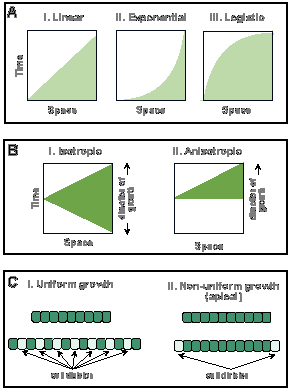
\includegraphics[width=0.8\textwidth]{chapters/Introduction/growth}
    \caption{\textbf{Components of biological growth.} \textbf{(A)} Growth functions can be linear (i) where growth rate is constant, exponential where growth rates increases over time (ii) or logistic where growth rates ultimately converges to zero (iii). \textbf{(B)} The direction of growth determines how the tissue evolves, where isotropic growth (i) has the same growth rates on all directions, while anisotropic growth has different growth rates in different directions. \textbf{(C)} Uniformity of growth depends on the growth rates of different regions of the tissue. For uniform growth (i), growth rates throughout the tissue are constant, meaning cell division occurs everywhere and tissue expands homogeneously. In non-uniform growth (ii), growth rates vary throughout the tissue such as apical growth where growth rates are only positive at the edges.}
    \label{fig:growth}
\end{figure}


Considering the importance of growth in pattern morphology, it is key to consider how this growth might affect parametric robustness in Turing pattern formation.
Interestingly, introducing slow isotropic growth allows certain network topologies to form Turing patterns, which would not without growth.
An example of that is patterns in activator-activator networks, showing growth induced Turing instabilities.
Additionally, short-range activation and long-range inhibition can also produce Turing patterning in growing domains~\parencite{gaffney2010}.
Finally, increasing growth rates can increase the Turing parameter space under exponential growth in Turing patterning networks.
However, the analytical analysis used in~\cite{gaffney2010} only holds when assuming slow isotropic growth and will break under faster growth.

Under logistic and linear growth, the Turing parameter space also changes.
However, the analysis used in~\cite{gaffney2010} only holds when assuming slow isotropic growth and will break under faster growths.
This analysis is revisited in~\cite{Klika2017} where they manage to study faster isotropic growing domains.
However, they observe that the conditions for Turing instabilities are more complex with higher growth rates and therefore more challenging to study than the ones in~\cite{gaffney2010}.
This complexity makes it difficult to carry out high-throughput studies of robustness and Turing parameter space in growing domains.
Finally, other types of growth such as anisotropic growth~\parencite{Krause2019} are studied, but again they do not study parametric robustness in detail.

\subsubsection{Boundary conditions}\label{boundary_conditions_intro}
Boundary conditions are a set of conditions that need to be satisfied at the boundary of a system where a set of differential equations is solved.
In reaction-diffusion systems, boundary conditions describe what happens to the morphogens as they reach a boundary.
In Neumann boundary conditions, the derivative at the boundary is defined.
If the derivative is zero, reflective boundary conditions are obtained (Fig.~\ref{fig:boundaries}B (top)).
In Dirilichet boundaries, the value at the boundary is defined.
Setting the value to zero creates an absorbing boundary where morphogens get leaked from the system (Fig.~\ref{fig:boundaries}B (bottom)).
Other boundaries such as periodic boundary conditions exist, where the morphogen passes through one boundary and appears in the other with the same velocity.
Biological systems can exhibit this wide variety of boundary conditions depending on the context and environment.
Additionally, these boundary conditions can also be replicated using experimental techniques~\parencite{Krause2020, Sheth2012, Vahey2014}.

\begin{figure}[H]
    \centering
    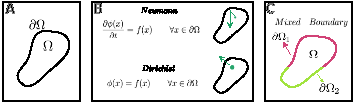
\includegraphics[width=1\textwidth]{chapters/Introduction/boundaries}
    \caption{\textbf{Boundary conditions.} \textbf{(A)} $\Omega$ represents the region governed by the differential equations and $\partial\Omega$ represents the boundary curve where the boundary conditions apply. \textbf{(B)} Neumann boundary conditions (top) are used to define reflective boundaries where the derivative is zero at the boundary. Dirilichet boundary conditions (bottom) are used to define absorbing boundary conditions where the value at the boundary is zero. \textbf{(C)} Mixed boundary conditions have a different boundary definition in different regions of the curve ($\partial\Omega_1$) and $\partial\Omega_2$)  }
    \label{fig:boundaries}
\end{figure}

Different theoretical studies explore a wide variety of boundary conditions for Turing systems.
Initially, it was shown that non-homogeneous boundary conditions where the system is not insulated (Dirilichet), are less sensitive to changes in the domain size, different initial conditions and perturbations in model parameters~\parencite{Arcuri1986}.
Then, mixed boundary conditions (Fig.~\ref{fig:boundaries}C) where different species are subject to different boundary definitions were also shown to increase parametric robustness~\parencite{Maini1993, Maini1997, Krause2021}.
Studying these effects of these boundary conditions analytically is relatively complicated as you need to understand the bifurcation from which the Turing instability arises.
For example, although a Turing bifurcation is canonically a pitchfork bifurcation under Neumann boundary conditions, the Turing bifurcation is canonically a transcritical bifurcation under Dirichlet boundary conditions~\parencite{Woolley2022}. %todo look at this again
This shows how much effect the boundaries have on the Turing instability, meaning they need to be considered when studying such systems.

A more applied biological example of how boundaries can affect pattern formation is seen in~\parencite{Krause2020} where they study patterning synthetic biofilm in agar plates.
In this case, the agar absorbs the diffusors through the boundary, disrupting the pattern formed in the biofilm.
This effect can be reduced by decreasing the thickness of the agar layer.
Potentially, the pattern could also be maintained by reducing the permeability of the agar through the introduction of a filter paper or reduction of pore size.

%todo add robustness upon prepatternur

%
%Indeed, the idea that biological systems exchange material with their immediate environment seems likely in many situations. Therefore no-flux boundary conditions might be irrealistic.
%(point sources in butterfly wings %todo cite murray 1981)

%    also boundary between two different types of cells may give rise to morphogen production at the boundary interface %todo~\parencite{meinhardt1981}.




\subsubsection{Noise}
Biological systems are known for their inherent noise.
Stochastic Turing patterns were studied by adding intrinsic noise in the production and degradation rates ~\parencite{Butler2009, Butler2011, Biancalani2010}.
In certain non-Turing parameter regimes, it was found noise could drive diffusion-driven instabilities.
If there is a stable mode with eigenvalues slightly below zero, noise can destabilise this mode leading to a noise-induced instability and therefore the emergence of a pattern.
More specifically, it was found that the requirements for large differential diffusivity between activator and inhibitor were relaxed.
This showed noise might be a source of parametric robustness, producing patterns where deterministic systems do not predict one.
However, the resulting patterns are not as ordered as deterministic Turing patterns~\parencite{Karig2018}.

Morphological robustness was also studied using intrinsic noise, which
stems from prescribing a probability that each reaction
occurs, rather than an exact rate.
It was shown analytically that stochastically excited wave modes correspond exactly to their deterministic analogues, leading to a similar final pattern.
Additionally, by perturbing populations away from the steady state, patterns formed quicker in a stochastic system than its deterministic counterpart~\parencite{Maini2012}


\subsubsection{Delays}
Gene expression delays also affect robustness for Turing pattern formation.
These delays stem from the lags of transcription, where mRNAs are produced from DNA reads; and translation, where proteins are synthesised from mRNA reads. These processes occur in the scales of minutes to hours, depending on the genomic size of the organism.
From a gene being activated to the protein being active, there is a delay that is often not accounted for when modelling patterning.
The pattern morphology has been shown to be extremely sensitive to delays including sensitivity to the initial conditions in the final pattern, dramatic changes in the patterning lag under different delays and even pattern loss when delays are introduced~\parencite{Maini2012, buchler2005nonlinear}.


Overall, it is important to understand how different phenomena can affect pattern formation and introduce in models the most relevant to the natural system or experimental system being studied.
Furthermore, in some cases, these biological phenomena could increase robustness to pattern formation and explain the lack of robustness found in classical Turing pattern studies~\parencite{Scholes2019}.
%
%\item Turing instability can appear through a pitchfork bifurcation (subcritical ) ---> l (Leppänen 2004; Benson et al. 1998;Crampin 2000;Dutt 2010, 2012; Grindrod 1996; Nicolis 1995; Auchmuty and Nicolis 1975; Bozzini et al. 2015; Breña-Medina and Champneys 2014; Dalwadi and Pearce 2022).  transcritical bifurcation
%Critically, the changes in bifurcation structure that are produced by altering the
%boundary conditions from Neumann to Dirichlet are not observed in the linear analy-
%sis,In this paper, we rectify this situation by demon-
%strating that although the Turing bifurcation is canonically a pitchfork bifurcation
%under Neumann boundary conditions (van Hecke et al. 1994), the Turing bifurcation
%is canonically a transcritical bifurcation under Dirichlet boundary conditions


\section{Engineering biological reaction-diffusion patterns}
Engineering Turing patterns involves building systems from first principles, based on Turing's reaction-diffusion mechanism, which can replicate natural periodic patterns.
To engineer biological Turing patterns specifically, cells and genetic components must be used to create the reaction-diffusion network.


There are various reasons to justify the engineering of Turing patterns in biology.
These justifications span from enhancing our fundamental understanding of how patterns develop in living organisms to the potential advancements these synthetic structures could contribute to biotechnology.

To begin with, there is a wealth of biological patterning that is associated with Turing-like gene networks, as indicated by numerous studies referenced in Section~\ref{Turing patterns in nature}.
However, due to the tangled nature of biological systems, it is extremely hard to prove a Turing’s mechanism is actually behind those biological patterns.
Building a biological patterning system based on the principles of Turing's mechanism would prove this mechanism can indeed form patterns in biology.
Furthermore, the integration of Turing patterns with real biological scenarios involving growth, stochasticity, or different boundary conditions could shift theoretical models towards more robust patterns that resemble more closely those found in nature.

Finally, the synthetic patterns obtained would contribute to novel nanotechnologies, such as systems with patterned biomaterial deposition~\parencite{Din2020, Cao2017}.
For this reason, a bottom-up approach is required to build a system from first principles, which is tunable and insulated from the tangled genetic context, and which can be used to build tissues of interest.



\subsection{Previous work on engineering spatial patterns}

Engineering Turing patterns in biology is a highly challenging endeavour that has required synthetic biology to gradually develop the appropriate tools.
This has involved creating simpler biological patterns, as well as chemical Turing patterns to gain the necessary insights and tools for this complex task.
In synthetic biology, a wide variety of pattern generators have been engineered ranging in different complexities and pattern outcomes.
To systematically categorise these synthetic patterning systems, we can group them into four levels based on design characteristics as described below and seen in Fig.~\ref{fig:engineered_patterns}~\parencite{huidobro}:


\begin{figure}[H]
    \centering
    \includegraphics[width=1\textwidth]{chapters/Introduction/SpatialComponentsFigure1_300dpi}
    \caption{\textbf{Engineered spatial patterns in synthetic biology.} This figure is adapted from our published review on synthetic spatial patterning~\parencite{huidobro}. Four levels of regulatory complexity in engineered spatial patterning systems. Each level is divided into an example circuit, and the resulting pattern upon implementation. Diffusing components of the circuit are labelled with a “D”, non-diffusing nodes are unlabelled. The colour of each node corresponds to the colour of the reporter in the respective implementation. Level 0: synchronized repressilator circuit implemented in a growing bacterial colony \parencite{Potvin-Trottier2016}. The plot shows the circuit oscillations in single cells or stirred liquid culture. Level 1: incoherent feedforward circuit, where the diffusor-producing sender cells (cyan) are placed in the middle of a bacterial lawn~\parencite{Basu2005}. The plot shows the concentration gradient of the diffusor away from the centre of the lawn. Level 2: self-activation and feedback inhibition circuit with one dynamically regulated diffusor creates spatial propagating waves and spatially synchronised oscillations (not shown)~\parencite{Danino2010}. The plot shows the oscillations of the circuit in single cells, or in a cell population. Level 3: self-activation and lateral-inhibition circuit with two dynamically regulated diffusors creates stationary Turing patterns in the TuIS chemical system~\parencite{Horvath}. The plot shows the localized, self-activating positive feedback of the slow-diffusing species D1 (blue curve) and the lateral inhibition of the fast-diffusing species D2 (yellow curve).} %TODO comment on adapted from literature
    \label{fig:engineered_patterns}
\end{figure}

Level 0 circuits lack synthetic signals that diffuse through normal Fickian diffusion, where the molar flux due to diffusion is proportional to the concentration gradient.
Instead, spatial structures emerge from other processes like cellular growth and gene expression freezing.
Examples include synchronised oscillator circuits in bacterial colonies producing periodic concentric ring patterns without diffusing signals~\parencite{Potvin-Trottier2016, Riglar2019} (See Fig.~\ref{fig:engineered_patterns} Level 0).

Level 1 circuits do rely on diffusible components; however, these are not dynamically regulated, meaning they are not produced by the circuit as it is in the case of Turing patterns.
These diffusors only act as a pre-pattern which the system will interpret~\parencite{Basu2005, Schaerli2014, Kong2017, Barbier2020, Grant2020}.
Although stripes and sharp boundaries can be obtained, their periodicity is limited.
Hierarchical patterning circumvents the periodicity issue by increasing the number of orthogonal diffusors used, which linearly increases the number of spatial domains~\parencite{Boehm2018}.
While hierarchical patterns can explain some developmental periodic patterns such as the neural tube in vertebrates~\parencite{Briscoe2015}, it fails to capture the self-organising periodicity of Turing patterns observed in development such as digit patterning~\parencite{Sheth2012,Raspopovic1} (see Fig. \ref{fig:engineered_patterns} Level 1).

Level 2 circuits do incorporate dynamically regulated diffusors; however, only one diffusor is introduced.
In contrast with level 1 systems, no pre-patterns are required to generate interesting behaviours.
Starting from a spatially homogeneous regime, these systems can produce robust spatial oscillators such as~\parencite{Danino2010} or simple single ring patterns~\parencite{Cao2016, Payne2013} (see Fig. \ref{fig:engineered_patterns} L evel 2).

Finally, level 3 circuits use multiple dynamically regulated diffusible components (see Fig.\ref{fig:engineered_patterns} Level 3).
Turing patterns are the most prominent example of Level 3 systems as they as formed by reaction-diffusion circuits of at least two diffusors.
While numerous robust systems have been engineered in Level 0,1 and 2 circuits, Level 3 or Turing pattern engineering are still in its infancy.
Stochastic Turing patterns were recently engineered in \textit{E.~coli} with a circuit implemented according to the self-activation and lateral inhibition topology, with two diffusible quorum-sensing signals~\parencite{Karig2018}.
Additionally, solitary patterns have also been engineered in a refactored Nodal–Lefty system in HEK cells~\parencite{Sekine2018}.
While easier to engineer due to their relaxed fine-tuning requirements, stochastic Turing patterns and solitary display more irregularity in their periodic spatial structure~\parencite{Butler2011, Karig2018,Sekine2018}.
x
While elusive in synthetic biology, regular-repeat Turing patterns have been engineered in chemical reaction systems.
They were first observed in the 1990's in the chlorite-iodide malonic acid (CIMA) reaction~\parencite{Castets, Lengyel1992} and later in the thiourea-iodate-sulfite (TuIS) reaction~\parencite{Horvath} (see Fig. \ref{fig:engineered_patterns} Level 3).
Unlike biological systems, chemical reactions are reliably described by the simpler laws of mass action, and system parameters can often be identified~\parencite{turanyi1994, kugler2009, Pusnik2019, Yeoh2019}.
Furthermore, the tuning of these systems by changing initial concentration or temperature has more predictable effects on the system~\parencite{Horvath, landeira2010, Asakura2011}.
Lastly, chemical systems are isolated from external interacting components unlike biological systems where burden and cross-talk between the cellular chassis and synthetic parts is inevitable~\parencite{Ceroni2015, Nielsen2016,Butzin2018, Du2020}.


Although chemical systems have helped understand pattern formation and could prove key to tissue engineering applications, mechanisms in biology seem to go beyond chemical systems.
Examples of patterns have been closely linked to gene expression patterns as shown in \textit{in-situ} hybridization studies~\parencite{Jing2006}.
For this reason, it is key to explore this avenue and build genetically based reaction-diffusion systems that generate robust periodic patterns in biofilms.


%todo comment that patterns are linked to gene expression because Modern experimental interrogations of suspected mor-phogen-based pattern formation systems, such as Nodal and Lefty zebrafish mesendodermal induction,use in situ hybridization [24–26]. This explicitly highlights local concentrations of specific mRNA tran- scripts and thus provides an indication of the rates of transcription of target genes, and emphasizes the role of gene expression in morphogenesis. Chen, Y. & Schier, A. F. 2002 Lefty proteins are long-
%range inhibitors of squint-mediated nodal signaling. Curr.
%Biol. 12, 2124–2128. (doi:10.1016/S0960-9822(02)01362-3)
%25 Jing, X. H., Zhou, S. M., Wang, W. Q. & Chen, Y. 2006
%Mechanisms underlying long- and short-range nodal
%signaling in Zebrafish. Mech. Dev. 123, 388–394.
%(doi:10.1016/j.mod.2006.03.006)
\subsection{Engineering Turing patterns in bacterial biofilms using exogenous circuit}
Even though they have been successfully engineered in chemical systems, the complexity of biology means that Turing patterns have never been engineered in a genetic context.
This can be attributed to the robustness problem including high sensitivity of parameters and a small fraction of parameter space producing Turing solutions.
Additionally, designing Turing circuits with the classical 2-node topology leads to constraints in differential diffusivity that hinder the engineering of Turing patterns.
Finally, this robustness issue is further amplified by the lack of orthogonal small-diffusible regulators to act as morphogens in a synthetic reaction-diffusion circuit.
Orthogonality refers to the inability of two or more molecules to interact with their respective substrates, so the activator or inhibitor functions work adequately.
%
%All these issues have been addressed by previous researchers in the Isalan Lab and myself to achieve the engineering of a synthetic Turing circuit in bacteria that can produce regular periodic stationary patterns.

To address the fine-tuning problem and differential diffusivity constraints,~\cite{Scholes2019} found that topology \#3954 was amongst the most robust 3-node networks in terms of kinetic parameters. %TODO ref topology if image is included
Additionally, this topology allowed for equal diffusivity and even faster diffusing activators.
A search around neighbours of the \#3954 topology was carried out to find that removing the positive feedback on node A did not decrease robustness substantially.
The resulting \#1754 topology seemed like a better candidate as it would be easier to build experimentally, while maintaining the robustness.
This topology is shown in Fig.~\ref{fig:synthetic circuit} (grey inset)

The lack of robust biological partly was addressed in~\cite{Meyer2019} and~\cite{Du2020} where orthogonal morphogens where characterized, which allow the building of the \#1754 topology.
These orthogonal morphogens are small quorum-sensing molecules which can activate gene expression by binding a promoter with high specificity, to activate downstream gene expression.
These toolboxes are key to bridge the gap between abstract models and real-sender receiver circuits.
Additionally, in~\cite{huidobro} we compiled a list of small molecule regulators that can diffuse and form gene circuits in \textit{E.~coli}, as well as their respective promoters and synthesis enzymes.
These could be investigated in the future to use as additional morphogens to build more complex systems with more diffusible molecules.

Finally,~\cite{Tica2020} engineered the \#1754 topology using the components from~\cite{Meyer2019} and~\cite{Du2020}, with the aim of exploring a Turing gene circuit for pattern formation (see Fig.~\ref{fig:synthetic circuit} bottom).
Due to the lack of specific biological parts such as an inhibitor quorum sensing molecule or a dual inhibitor/activator molecule, the biological implementation of \#1754 resulted in a six molecular species circuit instead of the original 3-node network.

\begin{figure}[H]
    \centering
    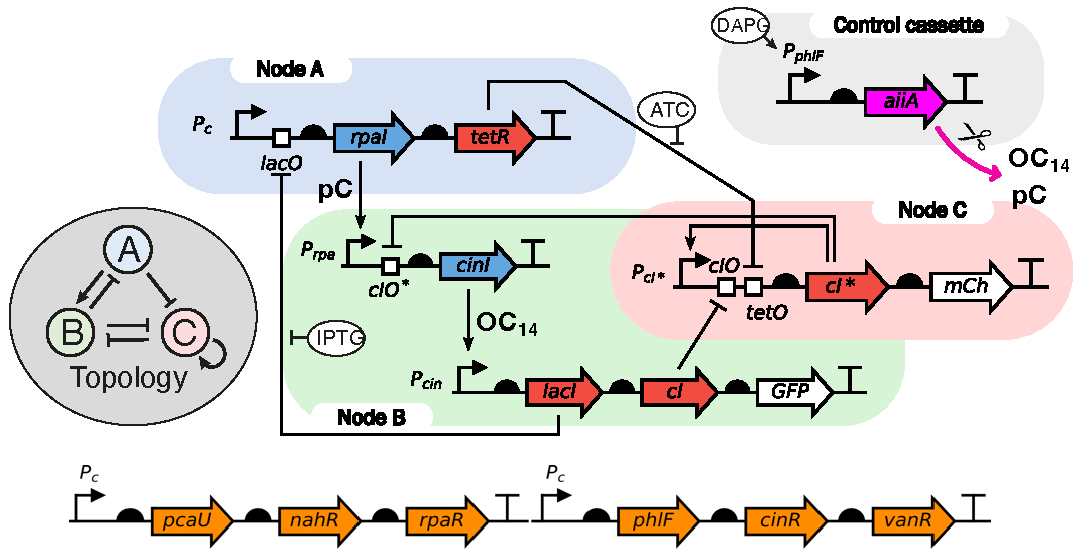
\includegraphics[width=1\textwidth]{chapters/Chapter 2/synthetic circuit2}
    \caption{\textbf{Synthetic biology implementation of \#1754 topology.} This synthetic circuit engineered by Jure Tica and Tong Zhu is a genetic abstraction of the \#1754 topology in \cite{Scholes2019}. This circuit is transformed so every \textit{E.~coli} cell in the biofilm has a copy inside. The original topology (left, grey inset) has only three nodes, while the synthetic circuit (right) has 6 nodes. The 6 gene circuit architecture, s hown in standard notation, can be clustered into the three original nodes as seen by the blue,green,red bubbles. Diffusor synthesis enzymes are in blue, non-diffusible transcription
    factors in red, fluorescent proteins in white. Diffusor synthesis enzymes produce quorum sensing molecules $pC$ and $OC_{14}$. The circuit can be regulated by small molecules ATC, IPTG and DAPG shown in white bubbles. DAPG activates the control cassette produces regulated degradation of small quorum sensing molecules. The bottom cassette (orange), contains the neccesary regulators: RpaR is the pC receptor (Node A diffusor), CinR is the OC14 receptor (Node B diffusor), and PhlF is the DAPG receptor (used to tune inducible diffusor degradation). The other three receptors PcaU, NahR and VanR are for the protocatechuate, salicylate and vanillin inducers, which are not used in the present circuit, but were tested in other versions of the system. These three systems can be used to introduce additional regulatory components to the system.}
    \label{fig:synthetic circuit}
\end{figure}

In this thesis, theoretical work based on this synthetic gene circuit was carried out to understand how to tune parameters experimentally and what spatial setup to use to allow pattern formation in bacterial biofilms.
Additionally, once the setup is determined, to predict which patterns might appear and the relevant wavelengths to look for.
Finally, once patterns appear in the biofilm, to characterise and understand the mechanisms behind these patterns.

Having a genetic synthetic network that produces patterns with a predictive model would be extremely impactful on various levels.
Firstly, the model would allow us to understand the patterning mechanisms behind the synthetic system and therefore shed some light into developmental biology.
Currently, our understanding from top-down approaches is based on arbitrarily chosen models that match well the experiments, but that are not directly informed on well-known and characterised gene circuits.
Model selection from those experiments is practically impossible as it has been proven that different models can generate the same 1D or 2D Turing pattern~\parencite{Woolley2021}.
In this bottom-up approach, the model used is derived from a known synthetic gene circuit that has been artificially introduced into cells.
This process constraints the model to provide more insightful results.
If this network can produce self-assembling periodic stationary patterns both~\textit{in-silico} and~\textit{in-vitro}, it would prove that a known reaction-diffusion system supported by genetic interactions can produce Turing patterns, therefore validating this mechanism.
Secondly, having a model would allow us to inform the experimentalists on how to tune the system to obtain more robust desired patterns or different shapes for tissue engineering in biotechnology applications.


\section{Thesis overview}

%%TODO mention chapter 1 and chapter 2 are a paper

This thesis explores Turing patterning within synthetic biology and tissue engineering, employing a modeling approach.
The novelty of this thesis lies in its modeling aspects, although it also includes some experimental results.

The first chapter adopts a theoretical perspective, delving into the relationship between linear stability analysis and numerical solutions.
Key aspects include estimating wavelength, convergence time, and, in some cases, predicting pattern shapes from the dispersion relation.
It also examines various instabilities capable of producing stationary spatial patterns beyond classical Turing instabilities.
This theoretical framework sets the stage for addressing realistic biological phenomena in pattern formation, such as varying boundary conditions and growth, crucial for understanding and engineering synthetic gene circuits for pattern formation.

The second chapter aims to develop a predictive model for the \#1754 topology, informed by the synthetic gene circuit outlined in~\cite{Tica2020}.
This PDE model is based on the interactions between genetic components and the diffusion of quorum-sensing molecules.
This model is used to explore the system's parameter space to identify regions prone to robust pattern formation and strategies for experimental tuning of the gene circuit.
Additionally, the model is parameterized using liquid culture data to determine its position within the parameter space.

The final chapter focuses on the experimental and modeling aspects of synthetic biofilms and their emergent patterns.
It presents initial experiments on small colonies forming periodic rings.
A PDE solver, combined with a cellular automaton for modeling bacterial colony growth, is then introduced, replicating all observed patterns, including spots, wedges, and rings produced by collaborators.
The chapter concludes with a detailed examination of the model's predictability against experimental perturbations, emphasizing the analysis of irregular growth, boundary effects, and node deletions.

In conclusion, this thesis significantly contributes to the fields of biology and mathematical biology, particularly in the realm of synthetic patterning.
By employing a predictive model and optimizing robustness, this work demonstrates the ability to guide experimental design for pattern formation as well as replicating the complex patterns obtained.
However, despite these advancements, the current level of robustness achieved remains relatively low, highlighting the need for further research.
Future work should focus on deepening our understanding of the underlying mechanisms and refining techniques to enhance the robustness and reliability of synthetic patterning processes.
This will be crucial in realizing the full potential of this technology in biomedical and industrial applications.

